\documentclass[12pt]{article}

\usepackage{graphicx}
\graphicspath{ {Fichier_Image/} }

\title{Hypothèses et validation ou non de ces dernières}
\author{Thibault Clodion}

\begin{document}

\maketitle % Permet d'afficher le titre, l'author etc

L'idée est ici de continuer à faire des expériences ayant pour but de valider ou refuter des hypothèses.
Après cela je pourrais mieux comprendre comment optimiser un bâtiment et adapter les résultats à un autre Cahier de Charge éventuellement.

\section{Hypothèses au propre}

\begin{enumerate}
    \item La taille des couloirs influe sur le temps de sortie
    \begin{enumerate}
        \item La taille des couloirs menant aux portes de sorties (juste devant) doit être la même que celle de la porte de sortie
        \item La taille de tous les couloirs doit être unique (pas d'effet entonnoir)
    \end{enumerate}

    \item La disposition des portes influe sur le temps de sortie, elles doivent être espacées pour gagner du temps

    \item Le nombre de porte par bureau influe sur le temps de sorties
    \begin{enumerate}
        \item Les bureaux du milieux ont besoin de plusieurs portes pour diminuer le temps de sorties
        \item Les petits bureaux doivent avoir qu'une seule porte pour diminuer le temps de sortie
        \item Certain bureaux (même grand) doivent avoir qu'une seule porte pour réguler les flux
    \end{enumerate}

    \item La taille des portes doit être la même que celle des couloirs pour diminuer le temps de sortie


    \item La taille des bureaux influe sur le temps de sortie (comme vu exp 1. + 4.-7.)
    
    \item Les croisements (carrefour) augmente le temps de sortie si il génère des flux opposés
    
    \item La disposition des meubles influent sur le temps de sortie.

\end{enumerate}


\section{Idée d'expérience pour Validation/Refutation des Hypothèses}

\begin{enumerate}

    \item
    \begin{enumerate}
        \item Je vais repartir de la simulation 1. et je vais proposer un couloir principal de taille 80cm, 1m, 1m25, 1m50, 2m
        \item Je garde le couloir principal selon le 1.a et je change la taille des autres couloirs en 80cm, 1m, 1m25, 1m50, 2m
    \end{enumerate}

    \item Mettre toutes les portes susceptible de créer deux flux opposés en collision en face les unes des autres et une autre simulation où ces portes sont espacées.
    
    \item 
    \begin{enumerate}
        \item Une expérience où les bureaux du mileux ont qu'une porte et une où ils en ont deux
        \item A partir de la 4., faire des simulations avec 1, 2, 3 portes par bureaux  
        \item Des simulations avec le bâtiment en photo, une où il a une porte (comme sur la photo) et une où il y en a deux dont une à gauche, donc il y aura plus de régulation des flux
        \newline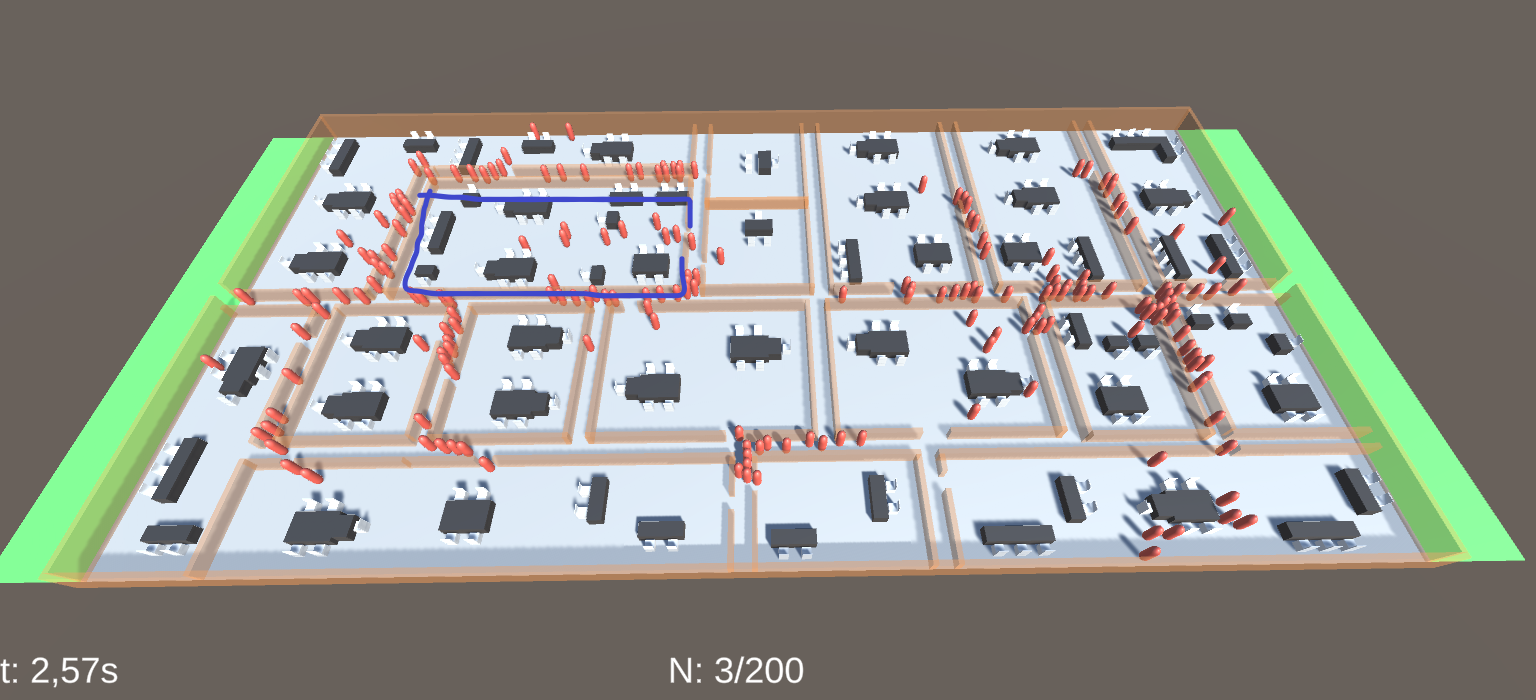
\includegraphics[scale=0.17]{7. bureau 1 porte.png}\newline
    \end{enumerate}

    \item Plusieurs simulations avec des portes de taille 80cm, 1m, 1m20, 1m50, 2m et des couloirs de taille fixe.
    
    \item Avec exp 1. et 4.-7. et d'autres expériences de ce genre montré que (grand bureau = grande densité proche des portes) et (grand bureau = possibilité de réguler les flux plis facilement) et (petit
    bureaux = moins de densité accumuler au même endroit).
    
    \item Enlever le carrefour exp 4. + Faire d'autre test de ce genre, où une simulation a un carrefour et l'autre non
    
    \item Plusieurs simulation, dont certaines où les meubles se situent dans les couloirs de circulation ou proche des portes et d'autres où les meubles sont espacés et laisse libre les portes + chemins.
    
    

\end{enumerate}

\section{Expérience et observations pour Validation/Refutation Hypothèses}

\begin{enumerate}
    \item 
    \begin{enumerate}
        \item On observe :
        \newline
        \underline{1.a -  Couloir Principal 80cm}
        \newline\newline
        \underline{1.a - Couloir Principal 1m}
        \newline\newline
        \underline{1.a - Couloir Principal 1m25}
        \newline\newline
        \underline{1.a - Couloir Principal 1m50}
        \newline\newline
        \underline{1.a - Couloir Principal 2m}

        \item On observe :
        \newline
        \underline{1.b - Autre Couloir 80cm}
        \newline\newline
        \underline{1.b - Autre Couloir 1m}
        \newline\newline
        \underline{1.b - Autre Couloir 1m25}
        \newline\newline
        \underline{1.b - Autre Couloir 1m50}
        \newline\newline
        \underline{1.b - Autre Couloir 2m}
    \end{enumerate}

    \item 

    \item    
    \begin{enumerate}
        \item 
        \item
        \item
    \end{enumerate}

    \item

    \item 

    \item 

    \item

    \item
\end{enumerate}

\section{Conclusion sur les Hypothèses}

\begin{enumerate}
    \item 
    \begin{enumerate}
        \item 
        \item 
    \end{enumerate}

    \item 

    \item    
    \begin{enumerate}
        \item 
        \item
        \item
    \end{enumerate}

    \item

    \item 

    \item 

    \item

    \item

\end{enumerate}

\end{document}